\subsection{Rayos x: Funciones de distribución de pares}

Se comienza caracterizando las estructuras amorfas obtenidas con el protocolo de litiación propuesto en la 
sección \ref{s:litpro} con las funciones distribución 
radial (RDF) parciales, que describen la probabilidad de encontrar un átomo de 
tipo B en un cascarón a una distancia $r$ de un átomo de referencia de tipo A y 
están definidas por la siguiente formula
\begin{equation}
    g_{AB}(r) = \frac{V}{4 \pi r^2 N_B} \sum_{i}^{N_A} \sum_{j\neq i}^{N_B} \delta(r - r_{ij}),
\end{equation}
donde $V$ es el volumen de la celda de simulación, $r_{ij}$ es la distancia entre
los átomos $i$ y $j$ y $N_A$ y $N_B$ son los números de átomos de tipo A y B, 
respectivamente. Estas curvas se muestran en la Figura \ref{fig:prdfs} para 
\begin{figure}[h!]
    \centering
    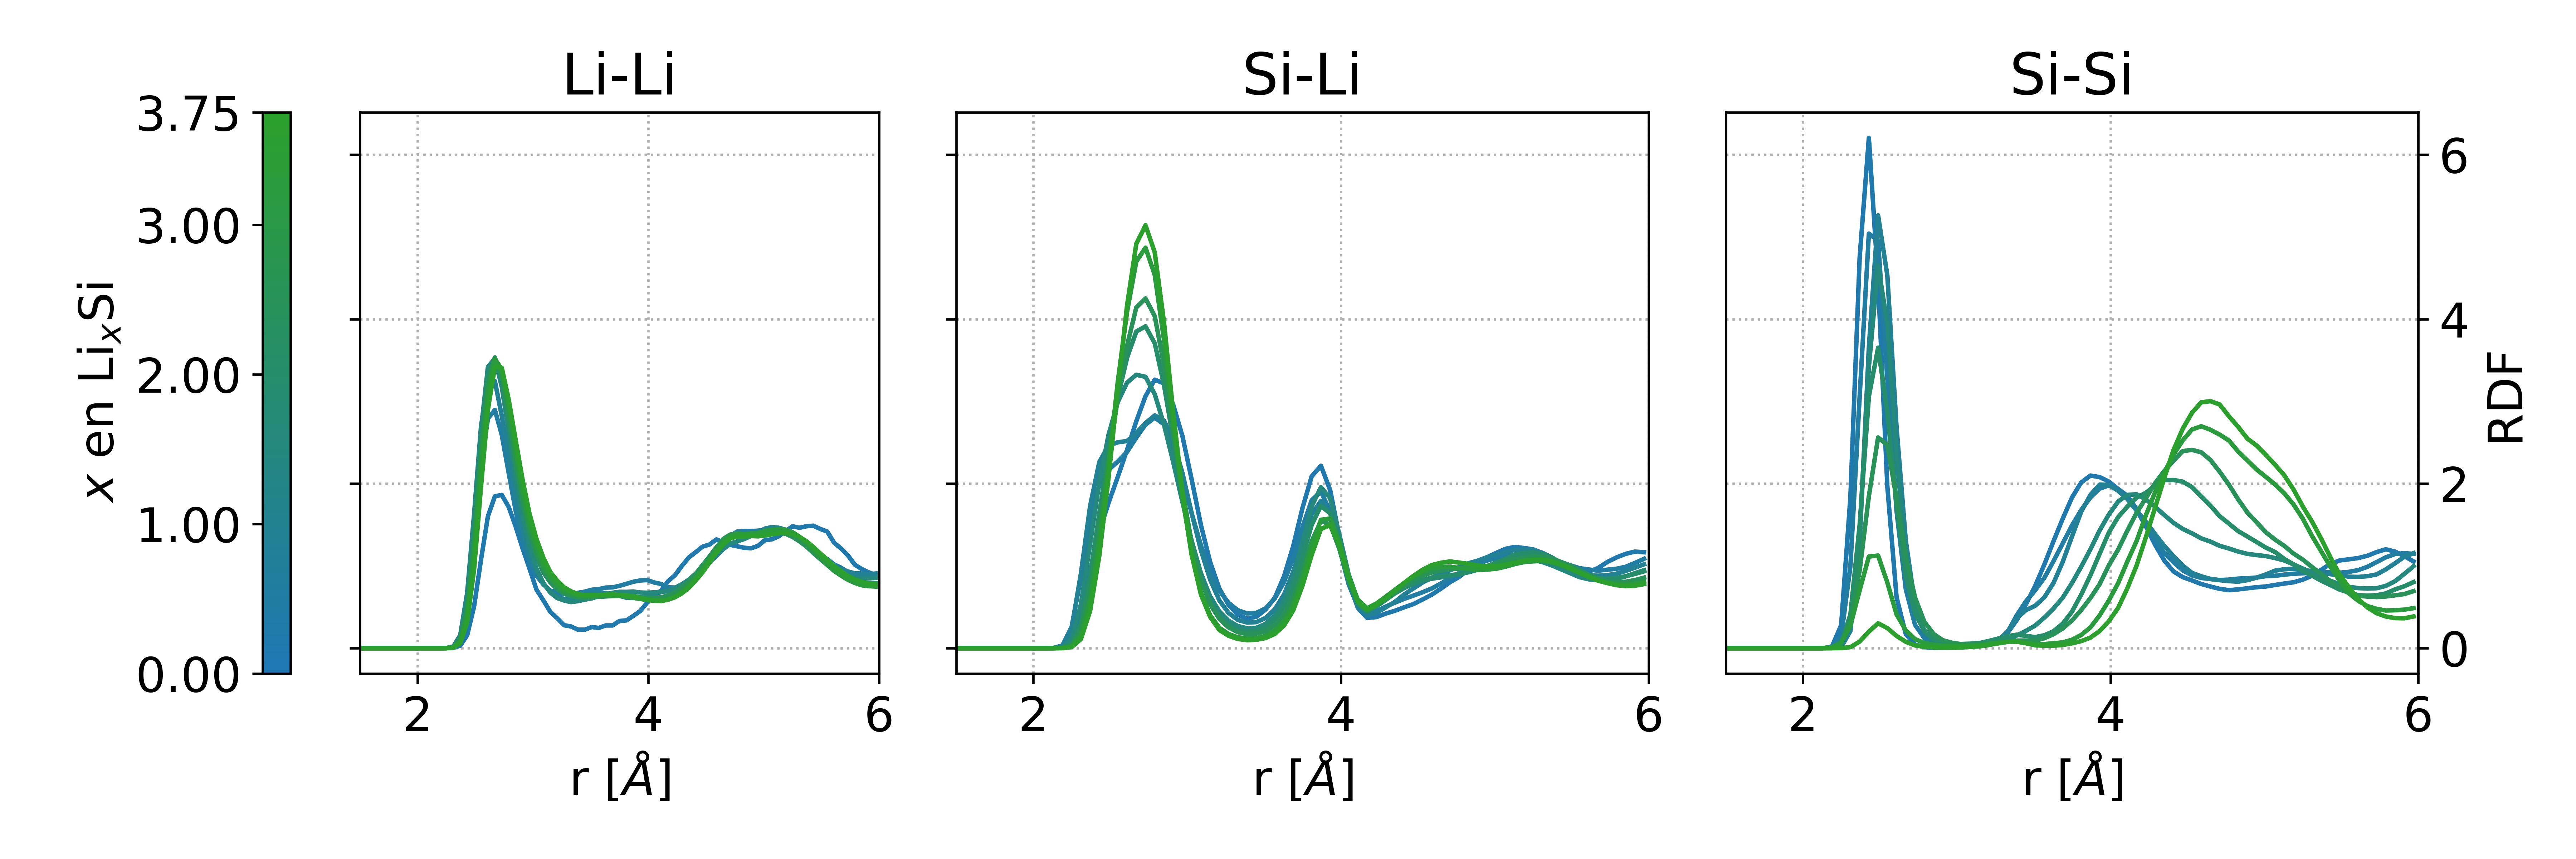
\includegraphics[width=\textwidth]{Silicio/prediccion/resultados/xray/prdfs.png}
    \caption{Funciones distribución radial (RDF) parciales para Li-Li, Si-Li y Si-Si para los valores $x$ en 
    Li$_x$Si optimizados (ver texto de sección \ref{s:litpro}). El color de la curva cambia de azul (predominio del Si)
    a verde (predominio del Li). Las barras de error son menores que el ancho de 
    las líneas.}
    \label{fig:prdfs}
\end{figure}
las distintas permutaciones de A y B (Li-Li, Si-Li, Si-Si); como puede observarse,
la naturaleza de las distribuciones calculadas es la típica de las estructuras
amorfas, presentando un primer pico bien definido a distancias cortas y picos 
decrecientes a medida que aumenta la distancia. Para el caso del Li-Li y del Si-Li
la forma de la distribución se preserva para los distintos valores de $x$ en 
Li$_x$Si. El comportamiento más interesante a analizar se encuentra en la RDF de 
Si-Si. Al aumentar la concentración de litio se aprecia una disminución del pico
correspondiente al primer vecino junto a un desplazamiento del segundo pico 
desde 3.8 \AA\ hacia 4.7 \AA. Esto indica que los enlaces Si-Si de la estructura 
amorfa inicial se rompen durante la litiación y aparecen Si aislados. Observando
con mayor detalle se aprecia un hombro en el segundo pico a distancias mayores 
a 5 \AA. Esto se relaciona con la persistencia de algunos enlaces Si-Si, es decir,
un Si aislado tiene un segundo vecino a 4.7 \AA. Si este último se encuentra 
enlazado a otro Si, entonces este se encuentra a una distancia de 5.0 \AA\ del 
primero. Cabe señalar que el modelo DFTB desarrollado en el capítulo 
\ref{ch:modelo} permite capturar estas características a un costo computacional
considerablemente menor que el que se tendría con DFT.

La combinación de las RDFs previas permite calcular la función distribución radial 
de a pares, $G(r)$, para cada estructura utilizando que \cite{billinge2019}
\begin{equation}
    G(r) = 4 \pi r \rho_0 \left[\sum_{\langle A,B \rangle} \frac{b_A b_B}{\langle b\rangle^2} g_{AB}(r) - 1\right], 
\end{equation}
donde $\rho_0$ es la densidad de la celda de simulación, $\langle A, B \rangle$
considera las permutaciones sin repeticiones de A y B, $b_A$ y $b_B$ son los 
factores de dispersión de los átomos A y B, respectivamente, y $\langle b \rangle$
es el factor de dispersión promedio de la celda de simulación. Los factores de 
dispersión para Li y Si son 3 y 14, respectivamente, lo que resulta en una 
contribución del 82\% para la RDF parcial de Si-Si, un 16\% para la Si-Li y
un 3\% para la Li-Li. La $G(r)$ puede ser directamente comparada con la PDF
obtenida de mediciones de rayos x. Los triángulos de la Figura \ref{fig:pdfs} 
se corresponden con mediciones de los casos extremos de Si amorfo (abajo) y
Si completamente litiado (arriba), las mediciones fueron reportadas por Laaziri 
\textit{et al.} \cite{laaziri1999} y Key \textit{et al.} \cite{key2011}, respectivamente.
\begin{figure}[h!]
    \centering
    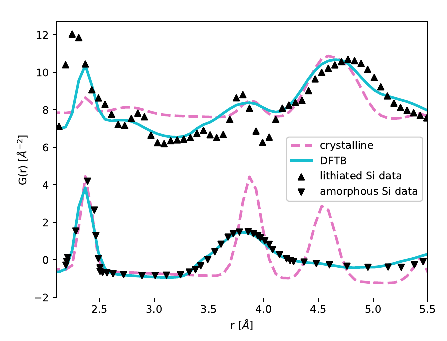
\includegraphics[width=.7\textwidth]{Silicio/prediccion/resultados/xray/pdfs.png}
    \caption{Funciones de distribución de pares $G(r)$ para Si amorfo y 
    completamente litiado contrastadas con datos experimentales. Los triángulos 
    que apuntan hacia abajo corresponden al experimento de a-Si de Laaziri 
    \textit{et al.} \cite{laaziri1999}, mientras que los que apuntan hacia arriba 
    corresponden al experimento de Key \textit{et al.} \cite{key2011}. Las curvas 
    DFTB azules consideran tanto las estructuras cristalinas y amorfas. Las 
    contribuciones de cada una están en la Tabla  \ref{t:w-gofrs}. Los datos del Si 
    litiado tienen una contribución extra de 8 \AA$^{-2}$ para tener las dos curvas 
    en el mismo gráfico. Las barras de error son menores que el ancho de las líneas.}
    \label{fig:pdfs}
\end{figure}
Los resultados obtenidos utilizando estructuras amorfas se muestran en color azul 
y se agrega en naranja, para comparar, lo que se obtendría si se consideraran sólo
estructuras cristalinas. Para el Si amorfo se grafica directamente la $G(r)$ 
promedio de la estructura simulada, resultando en una concordancia excelente con 
el experimento, como se observa en la parte inferior de la Figura \ref{fig:pdfs}.
Para el caso del ánodo de Si completamente litiado, se espera que la muestra 
experimental esté compuesta principalmente de Li$_{15}$Si$_4$ amorfo 
(a-Li$_{15}$Si$_4$), aunque también puede esperarse que haya una contribución 
cristalina (c-Li$_{15}$Si$_4$). Además, también es posible que presente una 
contribución de Si puro, debido a una litiación incompleta que resulte de varios 
factores experimentales como mala conectividad, eventos cinéticamente limitados 
o, incluso, una descomposición del Li$_{15}$Si$_4$ \cite{key2009, key2011}. Por 
lo cual, para la curva en la parte superior de la Figura \ref{fig:pdfs} se 
ajustaron los datos experimentales utilizando una combinación lineal de $G_s(r)$ 
de cada estructura $s \in \lbrace$c-Si, c-Li$_{15}$Si$_4$, a-Si,
a-Li$_{15}$Si$_4\rbrace$, de la siguiente manera 
\begin{equation}\label{eq:contributions}
    G(r) = \sum_s w_s \cdot G_s(r),
\end{equation}
donde cada $G_s(r)$ se presenta en la Figura \ref{fig:gofrs}. Para el 
ajuste de los pesos de las estructuras se minimizó el error cuadrático 
medio y se obtuvieron los valores que se presentan en la Tabla 
\ref{t:w-gofrs}.
\begin{figure}[h!]
    \centering
    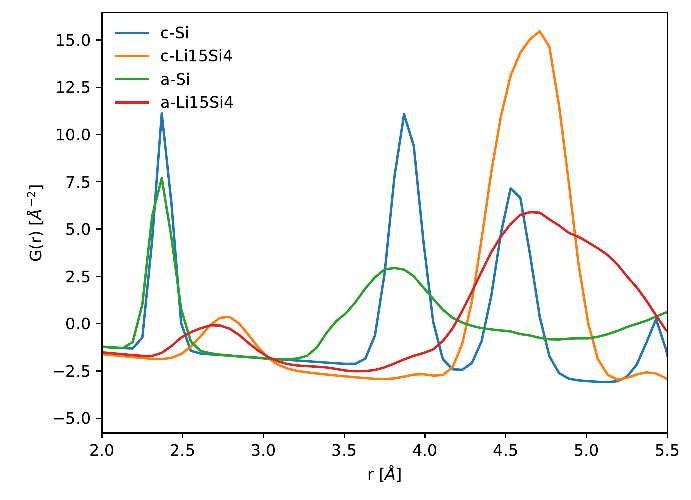
\includegraphics[width=.7\textwidth]{Silicio/prediccion/resultados/xray/gofrs.png}
    \caption{Funciones de distribución de pares $G(r)$ de estructuras 
    cristalinas y amorfas utilizadas para calcular las curvas de la Figura 
    \ref{fig:pdfs}.}
    \label{fig:gofrs}
\end{figure}
\begin{table}[h!]
    \centering
    \caption{Factor de peso de cada contribución (c-Si, c-Li$_{15}$Si$_4$, a-Si y 
    a-Li$_{15}$Si$_4$) a la función distribución radial de a pares $G(r)$ del 
    Si litiado (ver las Figuras \ref{fig:gofrs} y \ref{fig:pdfs} y la ecuación 
    \ref{eq:contributions}). El porcentaje que representa cada peso se agrega entre paréntesis.}
    \setlength\extrarowheight{2pt}\stackon{%
    \begin{tabular}{l c c c c}
        \toprule
        \textbf{Ajuste} & 
        \textbf{c-Si} & 
        \textbf{c-Li$_{15}$Si$_4$} & 
        \textbf{a-Si} & 
        \textbf{a-Li$_{15}$Si$_4$} \\ 
        \midrule
        DFTB amorfo & 0.0 (0.0\%) & 0.036422 (9.78\%) & 0.187971 (50.48\%) & 0.147955 (39.74\%) \\
        cristalino & 0.03358 (30.15\%) & 0.077784 (69.85\%) & -- & -- \\
        \bottomrule
    \end{tabular}
    }{}
    \label{t:w-gofrs}
\end{table}
Llamativamente, los pesos resultantes para las fases cristalinas son bastante 
pequeños, ya que representan el 9.78 \% para c-Li$_{15}$Si$_4$ y 0 \% para c-Si.
Esto destaca la importancia de considerar estructuras amorfas para entender 
determinaciones experimentales. Al contrario, si sólo se consideraran estructuras
cristalinas se tendría un ajuste considerablemente peor. Cabe destacar que, a 
pesar de que no se logran describir completamente algunas características de la 
PDF, existe una mejora significativa con respecto a un ajuste previo realizado por 
Key \textit{et al.} \cite{key2011}.
